\section{Referencia de la Clase Factura\-View}
\label{classFacturaView}\index{FacturaView@{FacturaView}}
Muestra y administra la ventana de una factura a cliente.  


{\tt \#include $<$facturaview.h$>$}

Diagrama de herencias de Factura\-View\begin{figure}[H]
\begin{center}
\leavevmode
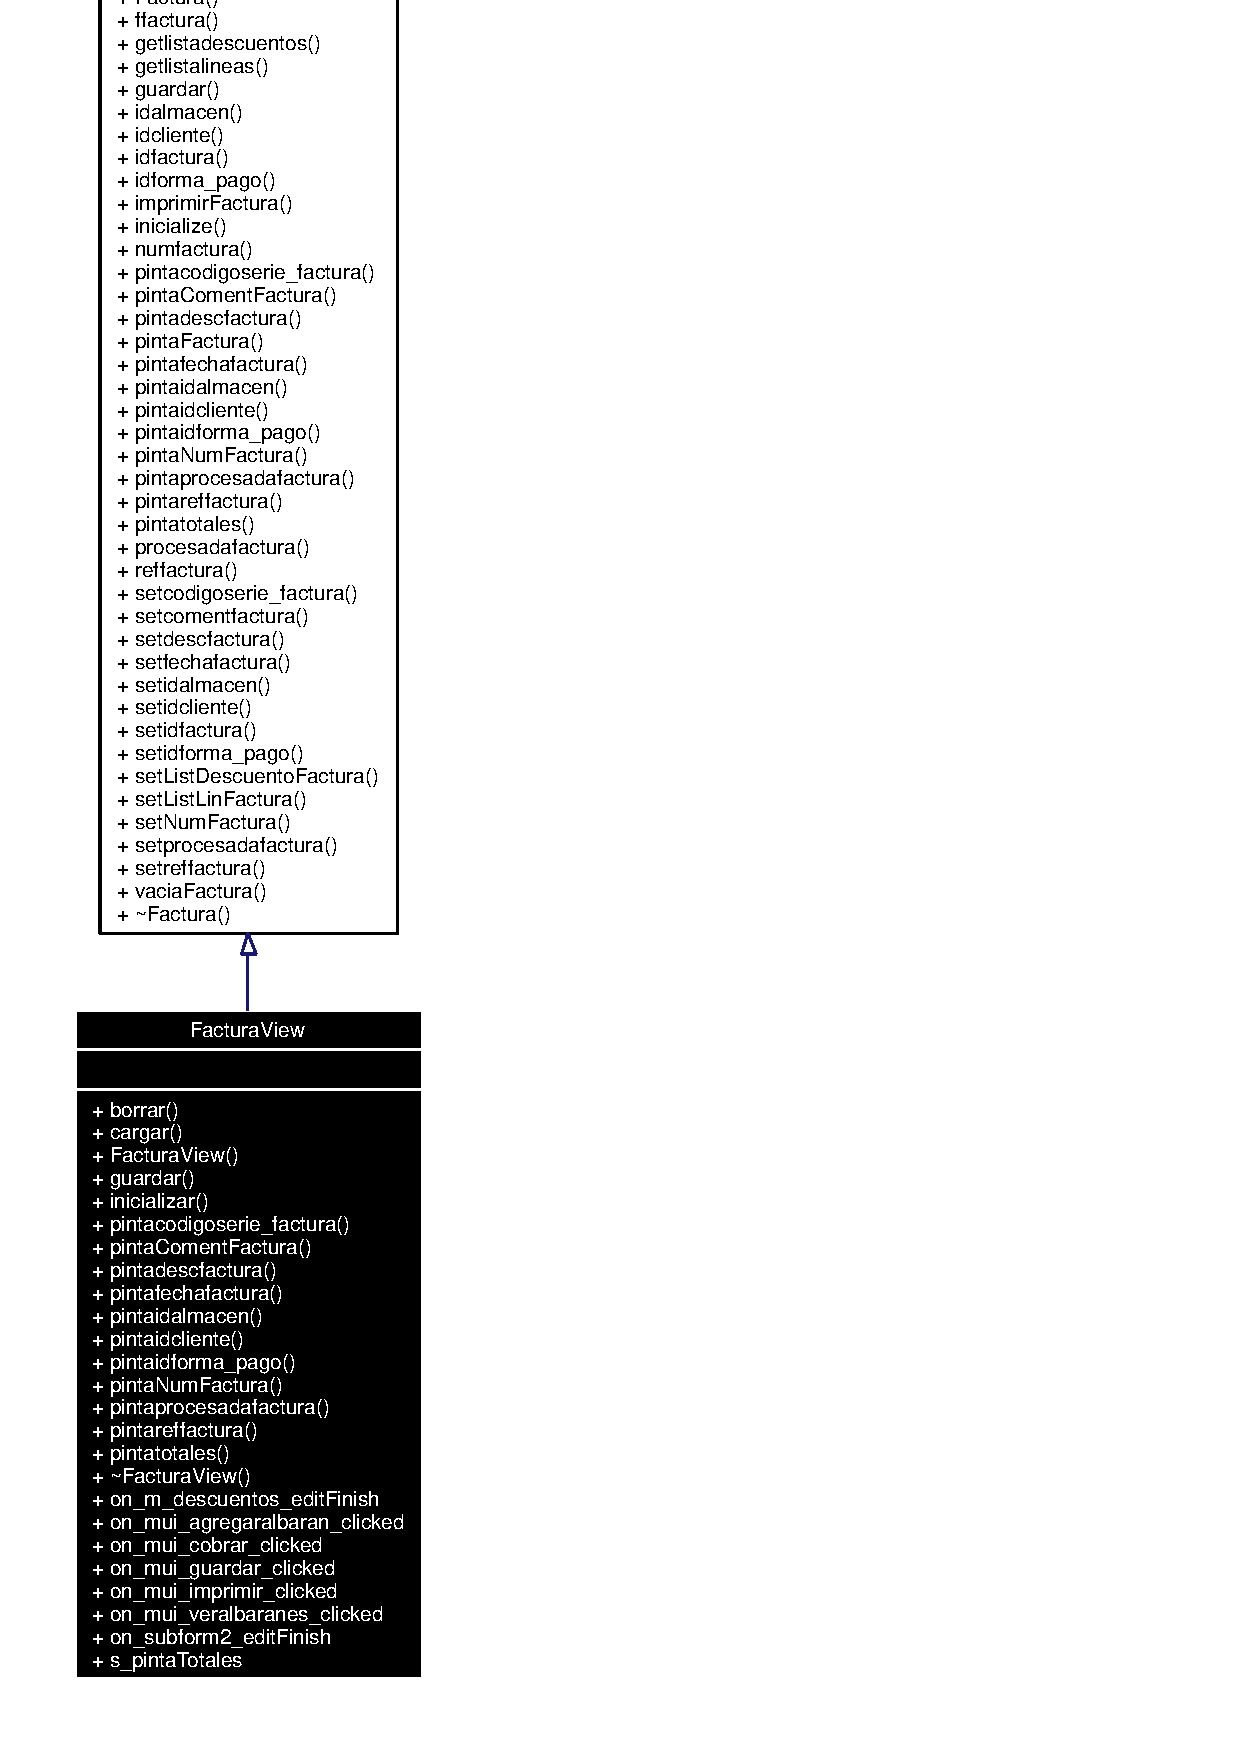
\includegraphics[width=101pt]{classFacturaView__inherit__graph}
\end{center}
\end{figure}
Diagrama de colaboraci\'{o}n para Factura\-View:\begin{figure}[H]
\begin{center}
\leavevmode
\includegraphics[width=101pt]{classFacturaView__coll__graph}
\end{center}
\end{figure}
\subsection*{Slots p\'{u}blicos}
\begin{CompactItemize}
\item 
virtual void {\bf on\_\-m\_\-descuentos\_\-edit\-Finish} (int, int)\label{classFacturaView_i0}

\item 
virtual void {\bf on\_\-mui\_\-agregaralbaran\_\-clicked} ()
\item 
virtual void {\bf on\_\-mui\_\-cobrar\_\-clicked} ()\label{classFacturaView_i2}

\begin{CompactList}\small\item\em Crea un nuevo cobro para la factura seleccionada. \item\end{CompactList}\item 
virtual void {\bf on\_\-mui\_\-guardar\_\-clicked} ()\label{classFacturaView_i3}

\item 
virtual void {\bf on\_\-mui\_\-imprimir\_\-clicked} ()\label{classFacturaView_i4}

\item 
virtual void {\bf on\_\-mui\_\-veralbaranes\_\-clicked} ()\label{classFacturaView_i5}

\item 
virtual void {\bf on\_\-subform2\_\-edit\-Finish} (int, int)\label{classFacturaView_i6}

\item 
virtual void {\bf s\_\-pinta\-Totales} ()\label{classFacturaView_i7}

\begin{CompactList}\small\item\em Este slot se activa cuando hay cambios en los subformularios. \item\end{CompactList}\end{CompactItemize}
\subsection*{M\'{e}todos p\'{u}blicos}
\begin{CompactItemize}
\item 
virtual int {\bf borrar} ()\label{classFacturaView_a0}

\item 
virtual int {\bf cargar} (QString id)\label{classFacturaView_a1}

\begin{CompactList}\small\item\em Esta funcion carga un factura. \item\end{CompactList}\item 
{\bf Factura\-View} ({\bf company} $\ast$, QWidget $\ast$parent=0)
\item 
virtual int {\bf guardar} ()\label{classFacturaView_a3}

\begin{CompactList}\small\item\em Estos metodos deben existir para poder trabajar con la clase Ficha. \item\end{CompactList}\item 
void {\bf inicializar} ()\label{classFacturaView_a4}

\item 
void {\bf pintacodigoserie\_\-factura} (QString id)\label{classFacturaView_a5}

\item 
void {\bf pinta\-Coment\-Factura} (QString id)\label{classFacturaView_a6}

\item 
void {\bf pintadescfactura} (QString id)\label{classFacturaView_a7}

\item 
void {\bf pintafechafactura} (QString id)\label{classFacturaView_a8}

\item 
void {\bf pintaidalmacen} (QString id)\label{classFacturaView_a9}

\item 
void {\bf pintaidcliente} (QString id)\label{classFacturaView_a10}

\item 
void {\bf pintaidforma\_\-pago} (QString id)\label{classFacturaView_a11}

\item 
void {\bf pinta\-Num\-Factura} (QString id)\label{classFacturaView_a12}

\item 
void {\bf pintaprocesadafactura} (QString id)\label{classFacturaView_a13}

\item 
void {\bf pintareffactura} (QString id)\label{classFacturaView_a14}

\item 
void {\bf pintatotales} (Fixed, Fixed, Fixed, Fixed)\label{classFacturaView_a15}

\end{CompactItemize}


\subsection{Descripci\'{o}n detallada}
Muestra y administra la ventana de una factura a cliente. 



\subsection{Documentaci\'{o}n del constructor y destructor}
\index{FacturaView@{Factura\-View}!FacturaView@{FacturaView}}
\index{FacturaView@{FacturaView}!FacturaView@{Factura\-View}}
\subsubsection{\setlength{\rightskip}{0pt plus 5cm}Factura\-View::Factura\-View ({\bf company} $\ast$ {\em comp}, QWidget $\ast$ {\em parent} = {\tt 0})}\label{classFacturaView_a2}


Usurpamos la identidad de mlist y ponemos nuestro propio widget con sus cosillas. 

\subsection{Documentaci\'{o}n de las funciones miembro}
\index{FacturaView@{Factura\-View}!on_mui_agregaralbaran_clicked@{on\_\-mui\_\-agregaralbaran\_\-clicked}}
\index{on_mui_agregaralbaran_clicked@{on\_\-mui\_\-agregaralbaran\_\-clicked}!FacturaView@{Factura\-View}}
\subsubsection{\setlength{\rightskip}{0pt plus 5cm}void Factura\-View::on\_\-mui\_\-agregaralbaran\_\-clicked ()\hspace{0.3cm}{\tt  [virtual, slot]}}\label{classFacturaView_i1}


Hacemos que las opciones de filtrado del listado ya esten bien.

Lanzamos el dialogo.

Si no hay idfactura es que hemos abortado y por tanto cancelamos la operacion.

Creamos la factura.

Agregamos a comentarios que albaran se corresponde.

EN TEORIA SE DEBERIA COMPROBAR QUE LA FACTURA Y EL ALBARAN SON DEL MISMO CLIENTE, pero por ahora no lo hacemos.

Los registros vacios no se tienen en cuenta.

Procesamos el albaran.

Pintamos los totales. 

La documentaci\'{o}n para esta clase fu\'{e} generada a partir de los siguientes archivos:\begin{CompactItemize}
\item 
facturaview.h\item 
facturaview.cpp\end{CompactItemize}
